\section{Experimental Setup}
\label{sec:4}
In this section, we discuss how to design the framework for discovering related articles in the corpus. As described in section \ref{sec:3}, each article contains semantic data including title, summary and content, together with meta-data, which consists of category, keywords, release date and the number of words in the texts. The purpose of this section is to evaluate how the methods which are mentioned in section \ref{sec:2} work in effectiveness and efficiency together with different semantic data. Then the assessment of filtering method which reduces the number of candidates with combining the meta-data is analyzed. In other words, this section focuses on finding the answer of question 1 and 2.

In section \ref{sec:4.1} the theoretical feasibility and challenge is discussed. The definition of terms and notations which are used in the rest sections is brought forwards in section \ref{sec:4.2}. In section \ref{sec:4.3} we discuss the design of experiments according to the application scenarios and depict the architecture of the framework. Furthermore, the setup of experiments is described in section \ref{sec:4.4}, including the setup of dataset given to experimenting and the setup of alternative models. 

\subsection{Theoretical Feasibility and Challenge}
\label{sec:4.1}

All STS methods and VSM models which are introduced in section \ref{sec:2}, are usually applied for computing the semantic similarity between texts. However, our goal is to find related articles for given target articles. Foremost, the difference between the term \textit{similarity} and \textit{relatedness} must be understood. The terms \textit{similarity} and \textit{relatedness} are two separate concepts\cite{pedersen2007measures}. \textit{Similarity} is the measure which indicates how a text looks like another text semantically, while relatedness is a more general concept, which contain multiple notions, such as causal relationship, temporal relationship and the relationship shared the identical event or background. We illustrate the difference with two examples. 

\begin{description}
\item[Example 1] There are two pieces of news. One of them reports the football game of Euro Champions between FC Bayern and Real Madrid in 2014, while the other reports the football game of German Bundesliga between FC Bayern and Dortmund in 2015. Obviously, they are similar to each other semantically, because they share the same topic (football game) and the same subject (FC Bayern).Meanwhile, they are unrelated to each other. The reason is that the two games are held in the different seasons and the different competitions. Exactly, football games is quiet a kind of short-term and event-sensitive events. 
\item[Example 2] Case TBD. They are not similar, because they may share quieta few words and meaning. However, they are related, because the both are about the consequence of TBD. The prediction of relatedness requires knowledge of the background in this case.
\end{description}

From the two examples, we can draw a conclusion, that computing relatedness is much more complicated than computing similarity, because the machine must understand exactly how humankind understands the identities and the differences between two articles as well as the significant degree thereof. However, \textit{similar} documents and \textit{related} documents have a non-negligible intersection normally. Our task is derived from a scenario of reality that two related articles need to be assigned for every current article. Therefore, it is unnecessary to find all possible related articles but it is acceptable to find only a subset of them. From this goal, a way from computing \textit{similarity} to getting \textit{related} articles is feasible. 

Certainly, discovery related articles using similarity methods leads to bias. It means, that the framework prefers predicting related articles only with specific characteristics and consequently some articles will never be assigned, e.g. articles which have the identical background with the target. The bias and error analysis are discussed in section \ref{sec:5}.

\subsection{Definition and Notions}
\label{sec:4.2}

In the following sections, a series of concepts is mentioned frequently. In order to avoid ambiguity and misapprehension, the definition and interpretation of these terms are given in the following list.

\begin{description}
\item[Article] an instance of a piece of news or report, which contains the complete information or rather texts of title, summary and content as well as meta-data. Denoted as $D$.
\item[Document] a specific component of an article which refers to the string of content without any explicit declaration as well as the string of title or summary when an explicit declaration is given. Denoted as $d$.
\item[Candidate] any article, which needs computing similarity with the target article, within the historic corpus.
\item[Token] the elementary semantic unit of a document 
\item[Word] (in the n-gram models) the elementary semantic unit of a document, which consists of $n$ adjacent tokens. Denoted as $w_i$. 
\item[Vocabulary] the set of words which occur in the corpus. In VSMs, the vocabulary contains the words which occur in the corpus at least $k$ times (in our case, $k=5$), in order to reduce the dimension of document-term-vectors. 
\item[Term] the unique item of the vocabulary $V$ which is generated by the entire corpus. Denoted as $t_i \in V$. 
\item[Related-graph] the graph in which the vertices are connected to each other according to the recommendation relationship which is stored in the corpus. If a path with two vertices exists, the corresponding articles are regarded as related to each other with the length $h$ of the path. Denoted the two articles are related with \textbf{hop-$h$}.

\label{tab:def_terms}
\end{description}


\subsection{Architecture of Framework and Experiments Design}
\label{sec:4.3}

The high-level architecture of the framework was already depicted in figure \ref{fig:highlevel}. In this section, we explain how the framework predicts related articles and improves itself. 

The framework consists of four phases of preprocessing, model building, similarity computing and model updating. The architecture of the framework is illustrated in figure \ref{fig:unsupervised}. 

\begin{figure}[!htb]
    \centering
    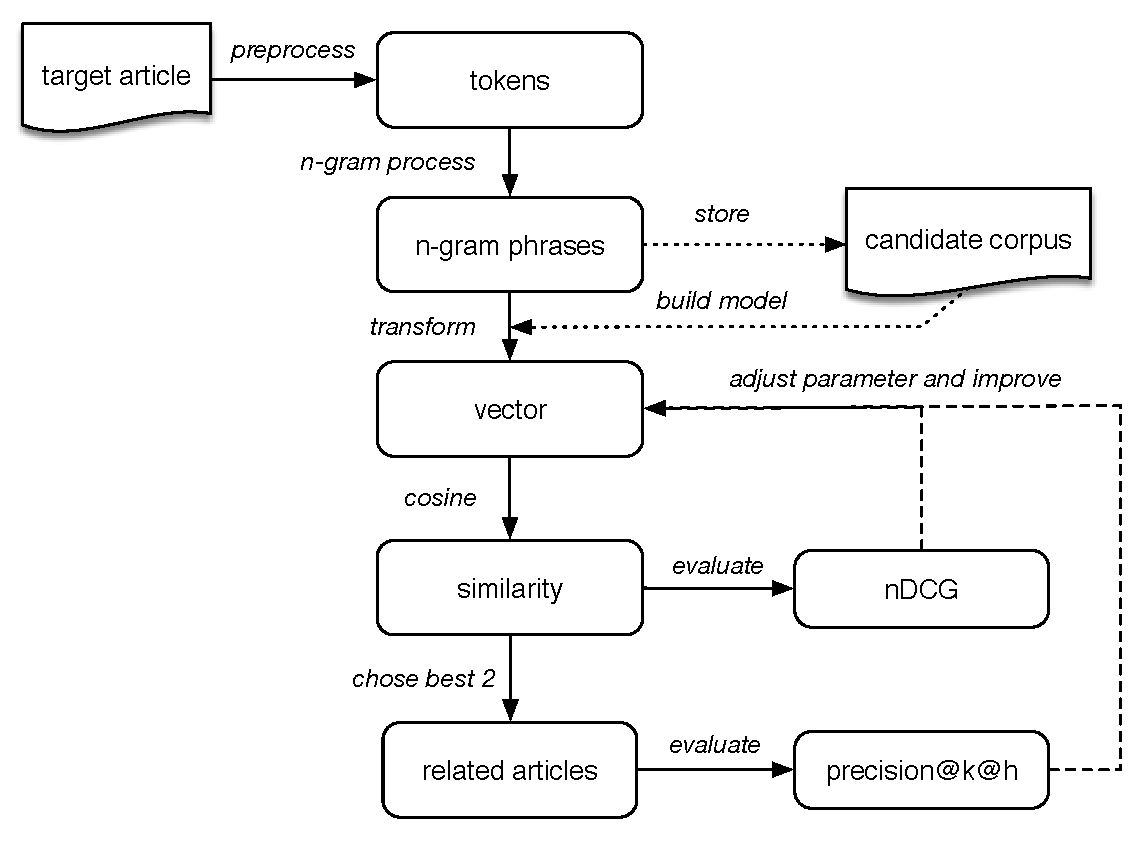
\includegraphics[width=0.7\textwidth]{fig/unsupervise}
    \caption{The architecture of the framework to discover related articles.}
    \label{fig:unsupervised}
\end{figure}


\subsubsection{Preprocessing}
The original data of title, summary and content is stored in the strings in HTML format. After all markups are removed and all characters are converted to small case, preprocessing separates the strings into the respective sequences of tokens. Four common methods are explained as follows:

\begin{description}
\item[\underline{SP}lit] The string is splitted into a sequence of tokens with the special characters (whitespace, hyphen and punctuations). 
\item[\underline{S}t\underline{E}m] Tokens, which are the result from the method \textit{SP} are replaced by the respective stems. For example, ``book'' is the stem of ``books'', ``booking'' and ``booked''. The advantage of stemming is to reduce the vocabulary size and decrease computational complexity and avoid overfitting of building semantic models. However, stemming causes the more serious problem of polysemy. 
\item[\underline{ST}op] After \textit{SP}, the stopwords, which are the most common words in a language, such as pronouns and prepositions are filtered out from the sequence. 
\item[\underline{S}tem+\underline{S}top] The data is handled by both of \textit{SP} and \textit{SE}. 
\end{description}

Preprocessing contains a sub-component, called n-gram processing. In our case, unigram, bigram and trigram are applied. In total, we have $4 \times 3 = 12$ alternative preprocessing methods. After preprocessing, the strings are represented as the respective sequences which the semantic models are able to deal with directly. 

\subsubsection{Model Building and Similarity Computing}
The component of model building is meaningful exclusive for VSMs. The approaches are quite different according to different models.  The detailed methods are described in the following list respectively.

\begin{description}
\item[BoW] BoW is the simplest and most basic model in VSMs. Each document is represented as a vector in which the weight of each dimension is the occurrence frequency of the respective term. In order to reduce the dimension of vectors, the terms which occur in the corpus at least $k$ times (in our case $k=5$) remain in the vocabulary. The BoW vector of a given document is independent of the rest corpus, so long as the vocabulary is constant. 
\item[tfidf] Tfidf is the model based on BoW, but the vector is relevant to the corpus. The tool to build tfidf model and the following models is \textit{gensim}\footnote{gensim is a NLP tool, which focuses on topic modeling and retrieving semantically similar documents \cite{rehurek_lrec}. Offical website: \url{https://radimrehurek.com/gensim/}}.
\item[LSI and LDA] We build the models LSI and LDA based on tfidf. Both models are capable to reduce the dimension of vectors from the vocabulary size to the number of topics. It is therefore necessary to determine the optimal number of topics, in order to make balance between the precision and computational performance. 
\end{description}

In VSMs, each document is transformed as a vector and the semantic similarity to other documents is the \textit{cosine} similarity between the vector of the target document and the vector of candidate documents. The articles in the historic corpus which are the most \textbf{two} similar to the given target article are predicted as the related articles. 

\subsubsection{Model Updating}

In the application scenario of reality, the historic corpus is not constant but increases over time. Once a article is ready to publish, the framework should select two articles with the greatest relatedness to the current article from the corpus. After the article is released, it should be stored into the historic corpus immediately and becomes the candidate for a related article to future articles. Therefore, the amount of the corpus will increase throughout. In the mean time, the characteristics of the corpus, for example, the topic distribution and the occurrence of new popular words, is rearranged over time. It is necessary thereby to update the model incrementally, in order to be able to reflect the recent situation of the corpus in time. However, the computational time cost of model updating must be taken into account. Accordingly, one of the research tasks is to find the trade-off between delay of updating and the impact on the performance of the effectiveness.  

\subsection{Experiment Description}
\label{sec:4.4}

TBD

We design two experiments to evaluate the framework. The first experiment focuses on the intrinsic performance of the different STS models with the different preprocessing methods. The intrinsic performance means the performance including effectiveness and efficiency that  The training corpus and the testing dataset are constant in the period of execution of the experiment. The purpose of the second experiment is to evaluate the fluctuate of performance when the size of the training dataset increases and the models need updating incrementally. In this case, an article is as the testing data at first and then is stored in the training dataset as the training data to update the models. 

\subsection{Hardware and Software}

The framework is set on a server running Linux system. The detailed information of the server is drawn in table \ref{tab:pcinfo}

\begin{table}[!htb]
%\centering
\begin{tabular}{ll}
CPU & Intel Xeon CPU E5420 (8 cores) @ 2.50GHz \\
RAM & 32GB \\ 
Disk & 3TB HDD \\ 
System & Debian GNU/Linux 7.7, 64 bits \\ 
Runtime & Python 3.4 \\
DBMS & MongoDB \\ 
Persistance & HDF5, gzip compressed \\
Externel Packages & NLTK, gensim, scikit-learn \\
\end{tabular}
\caption{General view of the hardware, system and software in use at major. }
\label{tab:pcinfo}
\end{table}


\begin{table}[!ht]
\begin{minipage}[b]{.45\linewidth}
\centering
\begin{tabular}{rrr}
\hline
\textbf{category} &   \textbf{quantity} &   \textbf{proportion (\%)} \\
\hline
Politik      &      26071 &            34.35 \\
Wirtschaft   &      12531 &            16.51 \\
Kultur       &       8584 &            11.31 \\
Gesellschaft &       7646 &            10.07 \\
Wissen       &       5273 &             6.95 \\
Sport        &       4993 &             6.58 \\
Digital      &       3887 &             5.12 \\
Reisen       &       2199 &             2.90 \\
Karriere     &       2169 &             2.86 \\
Studium      &       1570 &             2.07 \\
Lebensart    &        985 &             1.30 \\
\hline
\textbf{total}        &      75908 &           100.00 \\
\hline
\end{tabular}
\caption{Category distribution of \textit{ZEIT} corpus after filtering unsatisfied articles}
\label{tab:cate_dist_new}

\end{minipage}
\begin{minipage}[b]{.45\linewidth}
\centering
\begin{tabular}{rrr}
\hline
\textbf{year} &   \textbf{quantity} &   \textbf{proportion (\%)} \\
\hline
2009 & 12628 &            16.64 \\
2010 & 14716 &            19.39 \\
2011 & 13970 &            18.40 \\
2012 & 14583 &            19.21 \\
2013 & 14941 &            19.68 \\
2014 &  5070 &             6.68 \\
\hline
\textbf{total} & 75908 &           100.00 \\
\hline
\end{tabular}
\caption{Release date distribution of \textit{ZEIT} corpus after filtering unsatisfied articles}
\label{tab:release_dist_new}
\end{minipage}
\end{table}

\subsection{Dataset}

We setup the training and testing datasets from the ZEIT-corpus. Articles, which have no related articles or no \textit{title}, or whose content is less than 1000 characters, are filtered. Furthermore, articles which belong to a weak category \footnote{Weak category: the amount of articles in this category is fewer than $1\%$ of the corpus size} or which were released before 2009 are removed from the corpus. We have $75908$ articles in $7$ categories. The category distribution is drawn in table \ref{tab:cate_dist_new} and the release date distribution is in table \ref{tab:release_dist_new}




\begin{description}
\item[Experiment 1] $2000$ articles are selected randomly from the corpus as the testing dataset, and the others are as the history data to train the models. 
\item[Experiment 2] The articles in corpus are sorted by the \textit{release date}, so that the real-world scenario can be simulated. The articles, which were published before 2013, are as the training data to initialize models. There are two phases to deal with each target article, that are predicting related articles from the historical corpus and updating the model incrementally. Then the supervised methods make use of the scores from the unsupervised methods to compute the integrated scores and discover the related articles for each target article. 
\end{description}
